\chapter{Project Design}

\section{Software Requirement Specification}

\subsection{Hardware Requirements}
\\
\begin{itemize}
\item {2.4GHz Celeron Processor}
\item {256MB Memory}
\item {10GB Disk Space}
\end{itemize}

\subsection{Software Requirements}
\\
\begin{itemize}
\item {[Operating System]: Linux Based Operating System}
\item {[Build-essential]: Build-essential is required to build Debian packages, starting with dpkg (\textgreater= 1.14.18)}
\item {[Necessary packages for building GCC]:\\ \url{http://gcc.gnu.org/install/prerequisites.html}}
\end{itemize}

\subsection{Technologies Used}
\\
\begin{itemize}
\item C, lex, yacc.
\end{itemize}
\newpage
\section{U.M.L. Diagrams}
\paragraph{}
UML was meant to be a unifying language enabling IT professionals to model computer applications. The primary authors were Jim Rumbaugh, Ivar Jacobson, and Grady Booch, who originally had their own competing methods (OMT, OOSE, and Booch). Eventually, they joined forces and brought about an open standard. (Sound familiar? A similar phenomenon spawned J2EE, SOAP, and Linux.) One reason UML has become a standard modeling language is that it is programming-language independent. (UML modeling tools from IBM Rational are used extensively in J2EE shops as well in .NET shops.) Also, the UML notation set is a language and not a methodology. This is important, because a language, as opposed to a methodology, can easily fit into any company's way of conducting business without requiring change.
\paragraph{}
Since UML is not a methodology, it does not require any formal work products (i.e., "artifacts" in IBM Rational Unified Process lingo). Yet it does provide several types of diagrams that, when used within a given methodology, increase the ease of understanding an application under development. There is more to UML than these diagrams, but for my purposes here, the diagrams offer a good introduction to the language and the principles behind its use. By placing standard UML diagrams in your methodology's work products, you make it easier for UML-proficient people to join your project and quickly become productive. The most useful, standard UML diagrams are: use case diagram, class diagram, sequence diagram, state chart diagram, activity diagram, component diagram, and deployment diagram.

\paragraph{}
A \textbf{Use Case Diagram} in the Unified Modeling Language (UML) is a type of behavioral diagram defined by and created from a Use-case analysis. Its purpose is to present a graphical overview of the functionality provided by a system in terms of actors, their goals (represented as use cases), and any dependencies between those use cases. The main purpose of a use case diagram is to show what system functions are performed for which actor. Roles of the actors in the system can be depicted.
\paragraph{}
A \textbf{Sequence Diagram} in Unified Modeling Language (UML) is a kind of interaction diagram that shows how processes operate with one another and in what order. It is a construct of a Message Sequence Chart. A sequence diagram shows object interactions arranged in time sequence. It depicts the objects and classes involved in the scenario and the sequence of messages exchanged between the objects needed to carry out the functionality of the scenario. Sequence diagrams typically are associated with use case realizations in the Logical View of the system under development.
\paragraph{}
\textbf{Activity Diagram} in Unified Modeling Language (UML) is a kind of interaction diagram that shows how activities are carried out in synchronization with one another and in what order. It is a construct of a Flow Chart. A activity diagram shows object interactions arranged in time sequence. It depicts the objects and classes involved in the scenario and the activities exchanged between the objects needed to carry out the functionality of the scenario.
\newpage
\subsection{Use Case}
\begin{figure}[H]
\centering
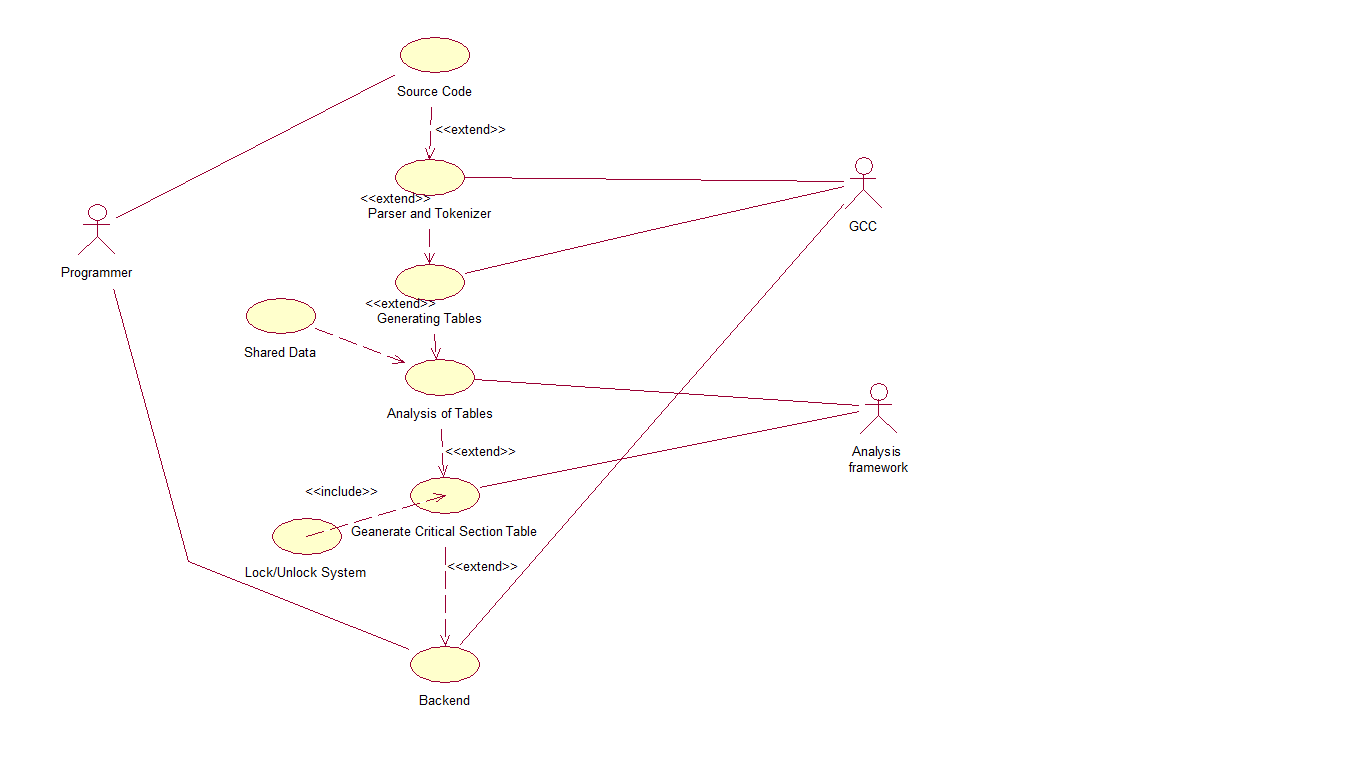
\includegraphics[scale=0.6]{usecase.png}
\caption{Use case diagram}
\label{<<Label>>}
\end{figure}
\paragraph{}
From use case point of view our system contains one actor as user or programmer, in which programmer has to specify a C source code (Source code should be error free and Multithreaded for better results).
And on the other hand GCC does the parsing and tokenization with the help of patterns and grammar that we have written, Analysis framework does the detection of critical sections in a source code provided by the Programmer as a input.


\subsection{State Chart}
\begin{figure}[H]
\centering
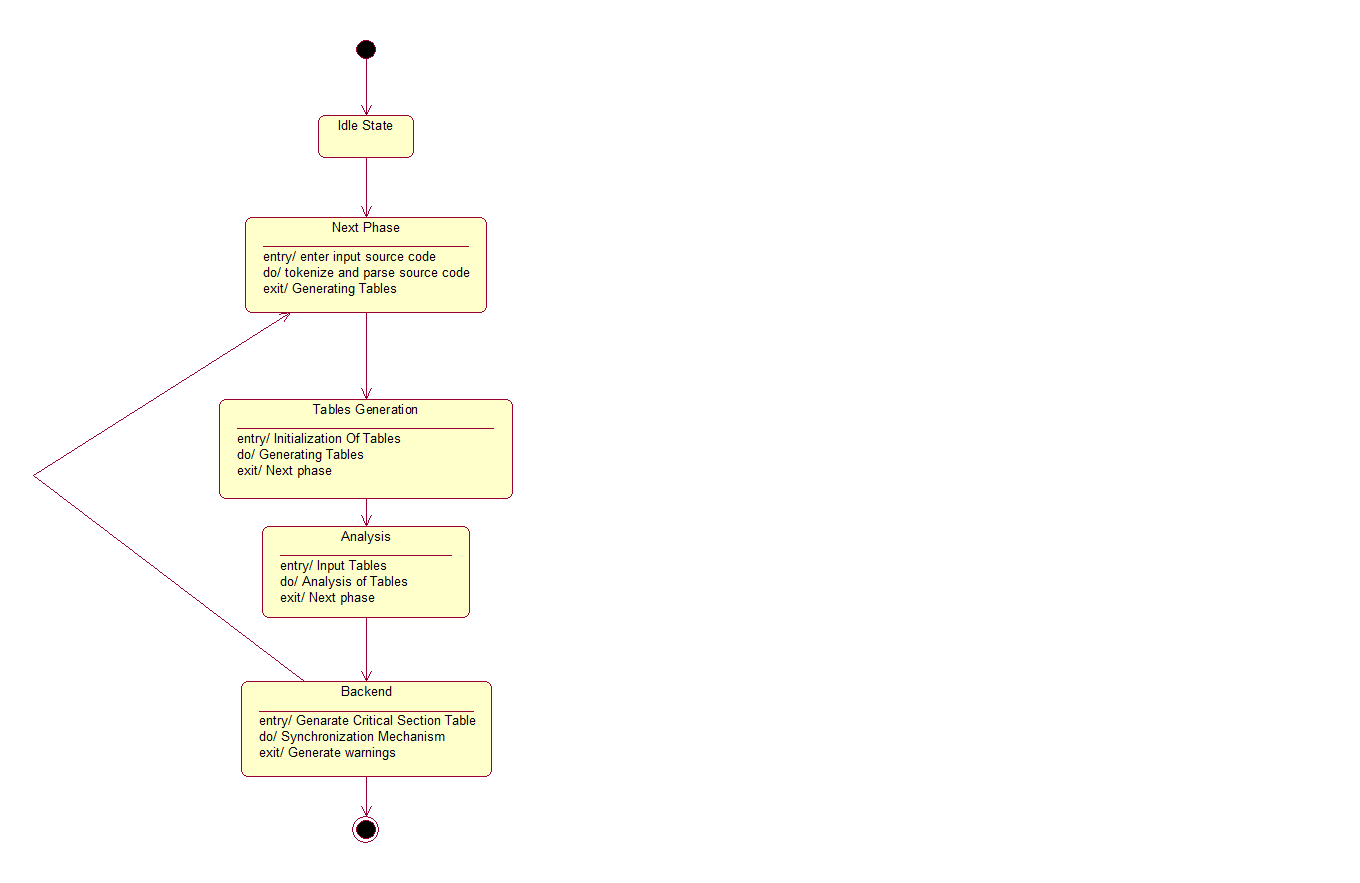
\includegraphics[scale=0.7]{statechart.png}
\caption{State chart diagram}
\label{<<Label>>}
\end{figure}
\paragraph{}
Control Flow of the Critical Section Detection System.
Above figure shows the state transisions of our system, this shows that how actually the system is going to transfer from eact step to next step after providing certain input. There are certain steps in each state. Flow of the Critical Section Detection System.

\subsection{Sequence Diagram}
\begin{figure}[H]
\centering
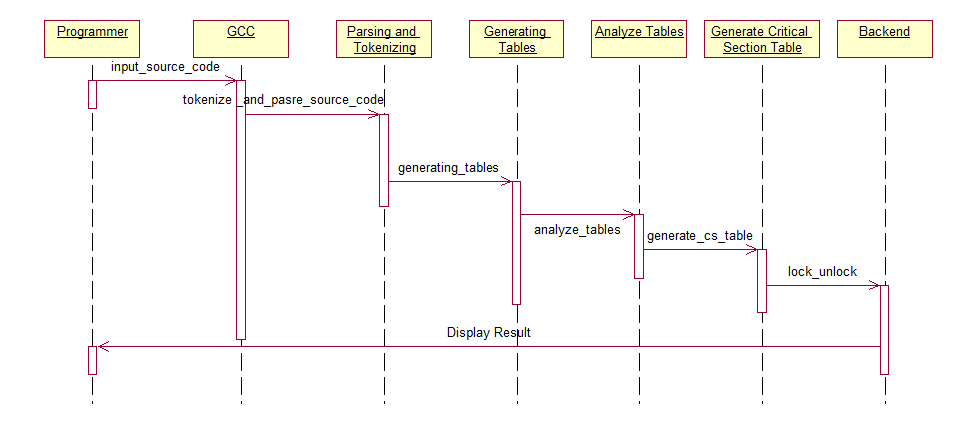
\includegraphics[scale=0.5]{sequence.png}
\caption{Sequence Diagram}
\label{<<Label>>}
\end{figure}
\paragraph{}
Shows the sequences of operations from starting to last one. A sequence diagram shows object interactions arranged in time sequence. It depicts the objects and classes involved in the scenario i.e Programmer, GCC, Analysis Framework etc. and the sequence of messages exchanged between the objects needed to carry out the functionality of the scenario. Scenario could be whole sequence of operations till the end result.  

\subsection{Collaboration Diagram}
\begin{figure}[H]
\centering
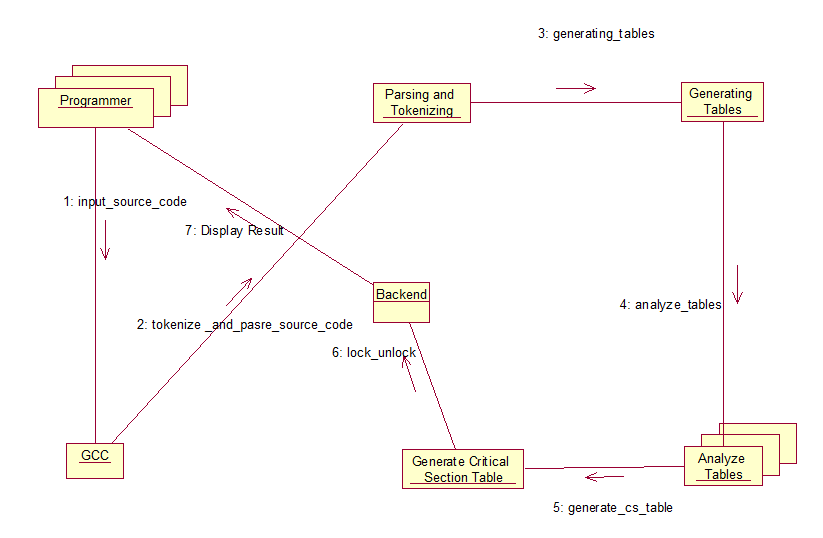
\includegraphics[scale=0.6]{collaboration.png}
\caption{Collaboration Diagram}
\label{<<Label>>}
\end{figure}
\paragraph{}
From Collaboarative perspective of our system, it covers the same scenario as shown in Sequence diagram.Indeed the collaborative view of the system is generated by using sequence diagram. 

\subsection{Activity Diagram}
\begin{figure}[H]
\centering
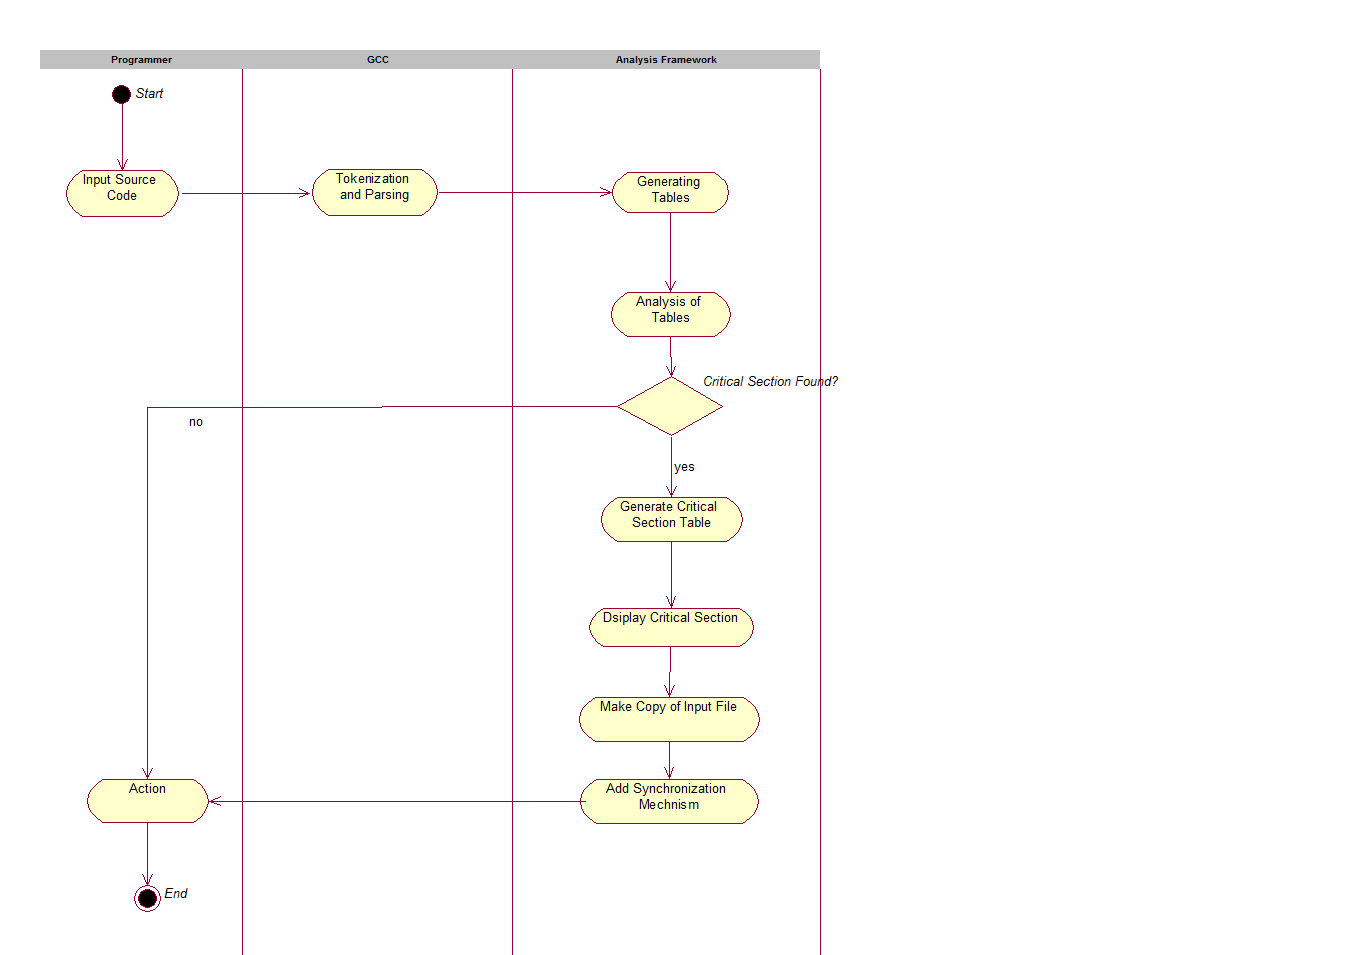
\includegraphics[scale=0.6]{activity.png}
\caption{Activity Diagram}
\label{<<Label>>}
\end{figure}
\paragraph{}
From programmers prespective activity diagram shows which are the diffrent activities performed by Programmer, GCC and the Analysis Framework.

\subsection{Component Diagram}
\begin{figure}[H]
\centering
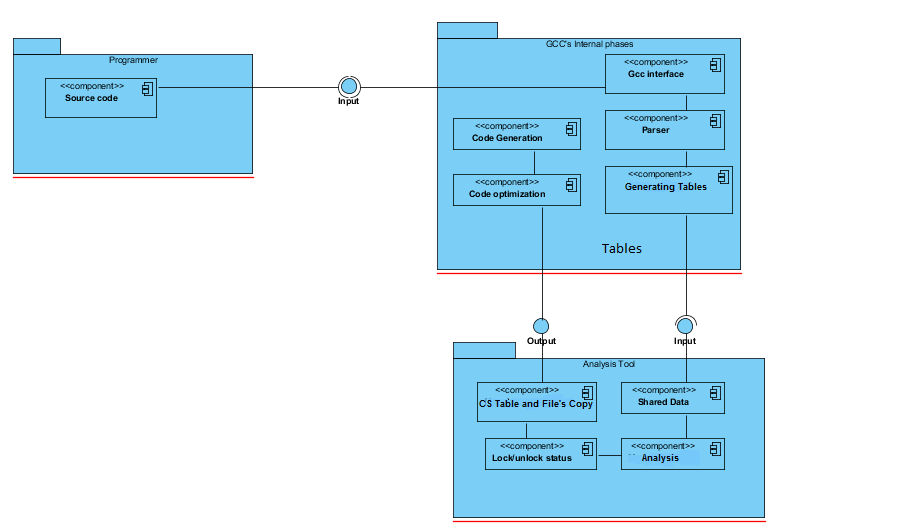
\includegraphics[scale=0.6]{component.png}
\caption{Component Diagram}
\label{<<Label>>}
\end{figure}
\paragraph{}
From Component point of view our system having different components used in system like system is Table Generator which generates the tables like Global Symbol's Table, Local Symbol's Table, Log Table, Semaphore Table, Function Table and Thread Table etc.

\subsection{Deployment Diagram}
\begin{figure}[H]
\centering
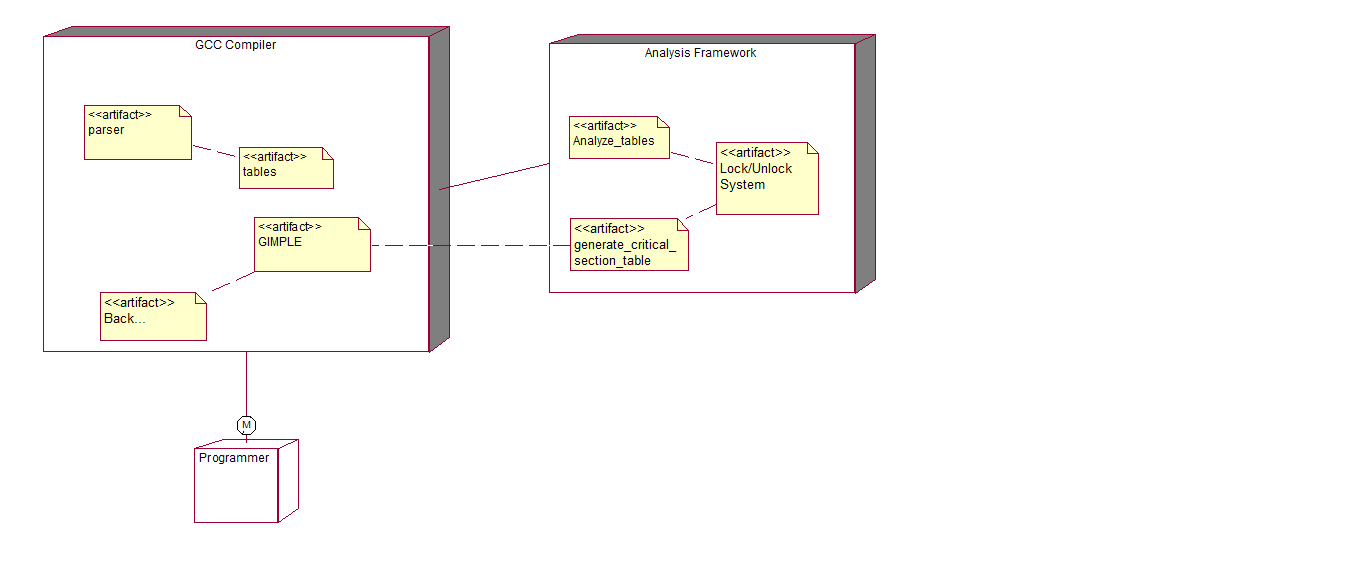
\includegraphics[scale=0.6]{deployment.png}
\caption{Deployment Diagram}
\label{<<Label>>}
\end{figure}
\paragraph{}
From deployment point of view our system contains following hardware and software component which are required for system execution are like GCC Compiler for compiling the source code, lex and yacc for Tokenization and Parsiing and the analysis frmaework for detecting the critical sections and adding synchronization mechanism.
